\part{Anexos}
% Anexo A
\chapter{Macros}
TeXstudio permite crear macros. El perfil tiene implementadas tres para facilitar la escritura de comandos para las siguientes acciones:
\begin{enumerate}
	\item Añadir hiperenlace.
	\item Añadir \textit{snippets} de código.
\end{enumerate}

Además de crear la macro, se han incluido en la barra de herramientas superior y se les ha puesto iconos específicos. También se han puesto iconos específicos para los botones del entorno \textit{equations}, en la barra de herramientas lateral.

% TODO: \usepackage{graphicx} required
\begin{figure}[h]
	\centering
	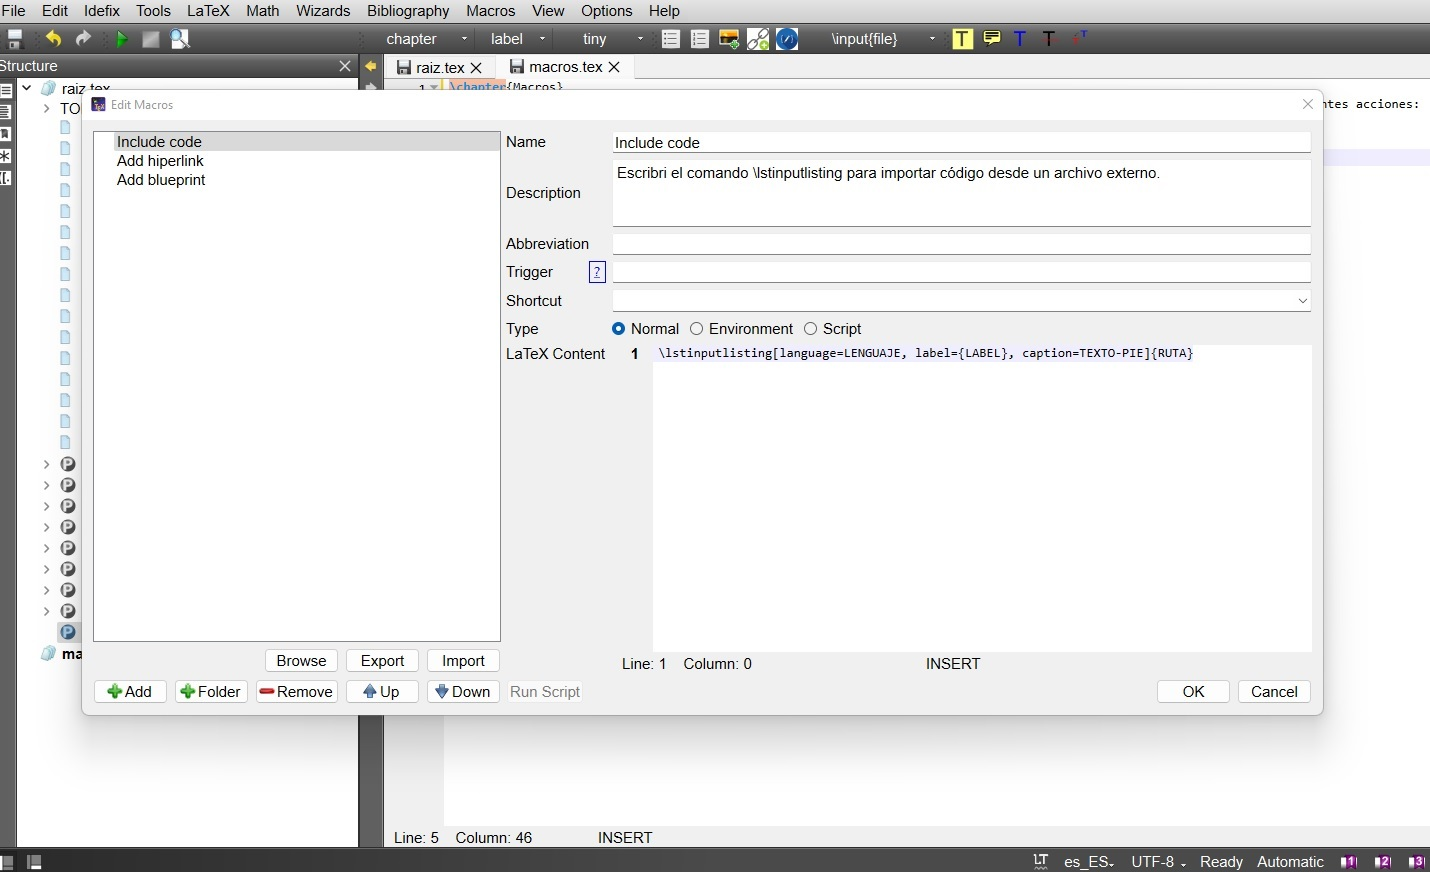
\includegraphics[width=1\linewidth, frame]{anexos/macros/imagenes/menu-macros}
	\caption[Menú Macros.]{Menú Macros. En este menú se pueden usar, crear y editar macros.}
	\label{fig:menu-macros}
\end{figure}

% TODO: \usepackage{graphicx} required
\begin{figure}[h]
	\centering
	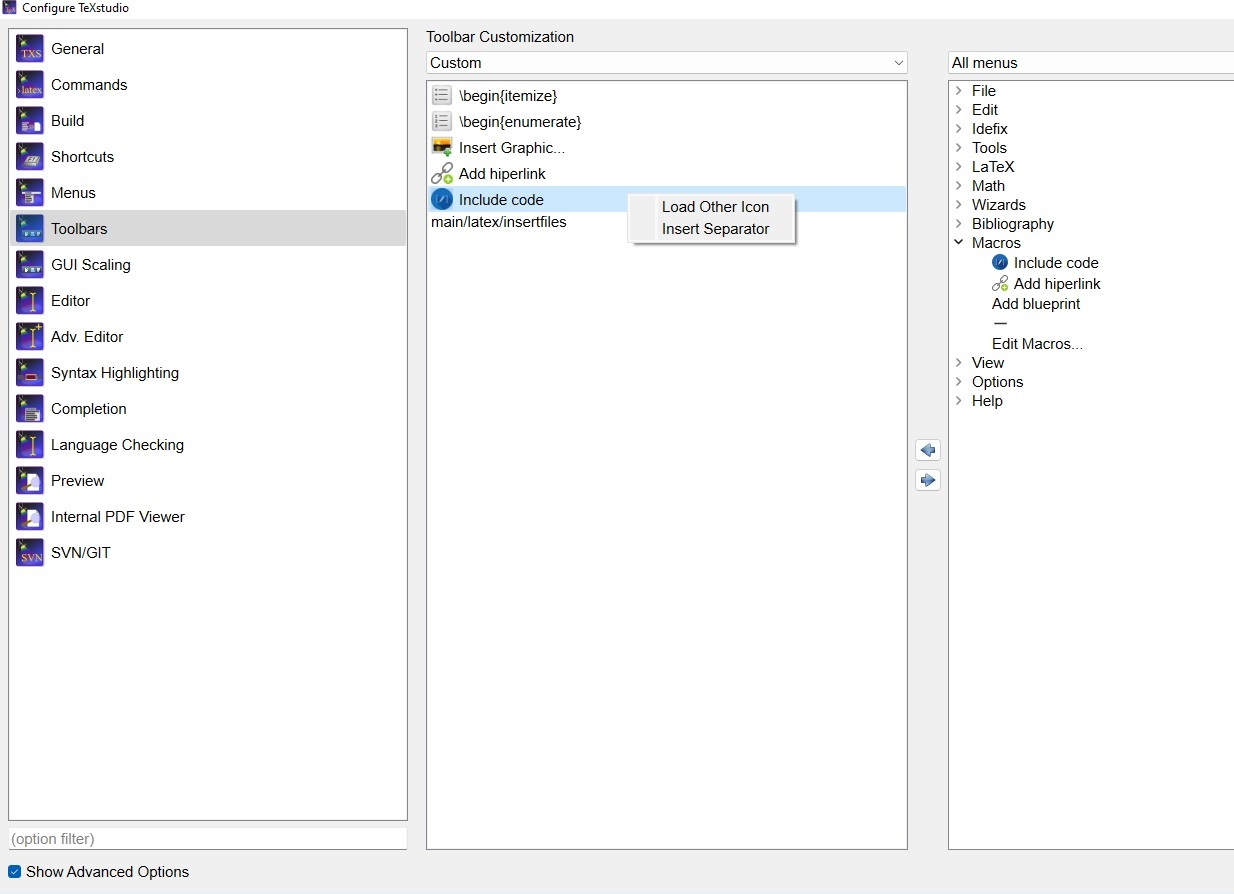
\includegraphics[width=1\linewidth, frame]{anexos/macros/imagenes/macros-boton-icono}
	\caption[Menú options/configuration/toolbars.]{Menú options/configuration/toolbars. En esta pantalla se pueden configurar las barras de herramientas, añadir botonoes e iconos.}
	\label{fig:macros-boton-icono}
\end{figure}

\begin{figure}[h]
	\centering
	
\includegraphics[scale=1, frame]{anexos/macros/imagenes/toolbar-sup}
	\caption[Barra de herramientas superior.]{Barra de herramientas superior. De izquierda a derecha los botones para las macros: tamaño de fuente, lista, enumeración, insertar imagen, insertar enlace, insertar código, insertar archivo; tras ellos botones para el paquete \textit{easyreview} para hacer comentarios de edición.}
	\label{fig:toolbar-sup}
\end{figure}

\begin{figure}[h]
	\centering
	
\includegraphics[scale=1, frame]{anexos/macros/imagenes/toolbar-lat}
	\caption[Barra de herramientas lateral.]{Barra de herramientas lateral. Los tres primeros botones, de arriba a abajo, son: entorno modo matemático, entorno ecuación numerada, entorno ecuación no numerada.}
	\label{fig:toolbar-lat}
\end{figure}

% Anexo B
\chapter{Comentarios con \textit{easyReview}}
El paquete \href{https://www.ctan.org/pkg/easyreview}{\textit{easyReview}} proporciona herramientas para realizar comentarios y revisiones, especialmente para trabajos colaborativos.

El perfil ya dispone de los botones para empelarla en la barra de herramientas superior (figura \ref{fig:toolbar-sup}).

\section{Ejemplo de uso de \textit{easyReview}}
Lorem ipsum dolor sit amet, consectetur adipiscing elit \alert{este texto es una alarma}. Aenean egestas quis felis vel volutpat. \comment{Vestibulum tincidunt}{Esto es un comentario a Vestibulum tincidunt; Se añade al índice de Todo´s} quam ligula, vel efficitur sem suscipit eu. Etiam tortor ligula, luctus ut mattis quis, varius facilisis neque. Nullam cursus metus ac accumsan semper \add{Esto es un texto a añadir}. In tincidunt vel elit sit amet semper. Nullam aliquam massa urna, a posuere ex scelerisque ut. Maecenas iaculis \remove{esto es un texto a eliminar} mi vitae turpis imperdiet mollis. Donec accumsan eu sapien eget mattis. Morbi nec maximus tortor, eget sagittis tortor. \replace{Pellentesque sodales}{este es el texto sustituto del tachado Pellentesque sodales}, mi ut dapibus malesuada, ipsum ipsum efficitur neque, in consequat dui sapien quis sapien. Mauris eros odio, ullamcorper at metus id, vestibulum pharetra sapien. Integer non purus sit amet diam faucibus blandit finibus non ex. Cras at lorem eget tortor malesuada ullamcorper. Praesent ipsum enim, laoreet sit amet quam non, imperdiet dignissim nibh. Duis ac sollicitudin tellus.
%
%	------------------------------------
%COD	GLOSARIOS
%-	------------------------------------
% Al estar tras la declaración de inicio de anexos, los glosarios se consideran como anexos. Al definir cada glosario como un capítulo (\chapter) cada uno es un anexo.
% Glosario de términos:
\printunsrtglossary
% Glosario de siglas y abreviaturas:
\printunsrtglossary[type=\acronymtype, title=Siglas y Abreviaturas, toctitle=Siglas y Abreviaturas]
% Glosario de símbolos
\printunsrtglossary[type=symbols, title=Listado de símbolos, toctitle=Listado de símbolos]